\section{Target of evaluation}
\label{sec:target-evaluation}

For the purposes of this report, the Tribunal of Bengodi provided us with a network scan of their premises. We used the available data to draw a preliminary mapping of their network in order to ease later work

Figure \ref{fig:initial-network} shows the state of the network. Since the scan was partially complete, we had to make several assumptions and edit the diagram slightly.

Floors are represented by the dotted circles. The leftmost one is the $1^{st}$ floor, the topmost one is the $2^{nd}$, the rightmost one is the $3^{rd}$, while the remaining small one is the ground floor. Thick black lines represent trunk connections between the default gateway and floor switches. We decided to address the lack of gateway IPs in some VLANs by adding a fictional firewall/router, whose networks are connected with light grey lines. Finally, this router is connected to the Prosecutor Investigator Labs and marked as \textit{Scanner Location}.

The rest of the diagram is fairly straightforward and uses VLAN tags along with color markings for better understandings of VLAN locations. The VPN access is located in the bottom right, connected to the Civil Court Clerks subnet (VLAN \verb=17=).

This approach, if left untouched, presents multiple flaws. Firstly, as it stands it's unclear whether traffic going to and from the VPN concentrator will be firewalled or will take a different route. This must be addressed first. Secondly, the VLAN \verb=17= is shared with the Prosecutor Head and Assistant subnet. Since we don't know if the two VLAN can contact each other (i.e. if there's a router segmenting them or not, which is hard to know with a simple scan), we need to make sure to segment the two into separate VLANs. This approach must be taken for all conflicting subnets (i.e. VLANs \verb=18, 40, 53=).

As it stands, deploying a VPN on such an architecture would be detrimental to security. In Section \ref{sec:summary-findings}), we propose some mitigations to this deployment.

\begin{figure}[!h]
	\centering
	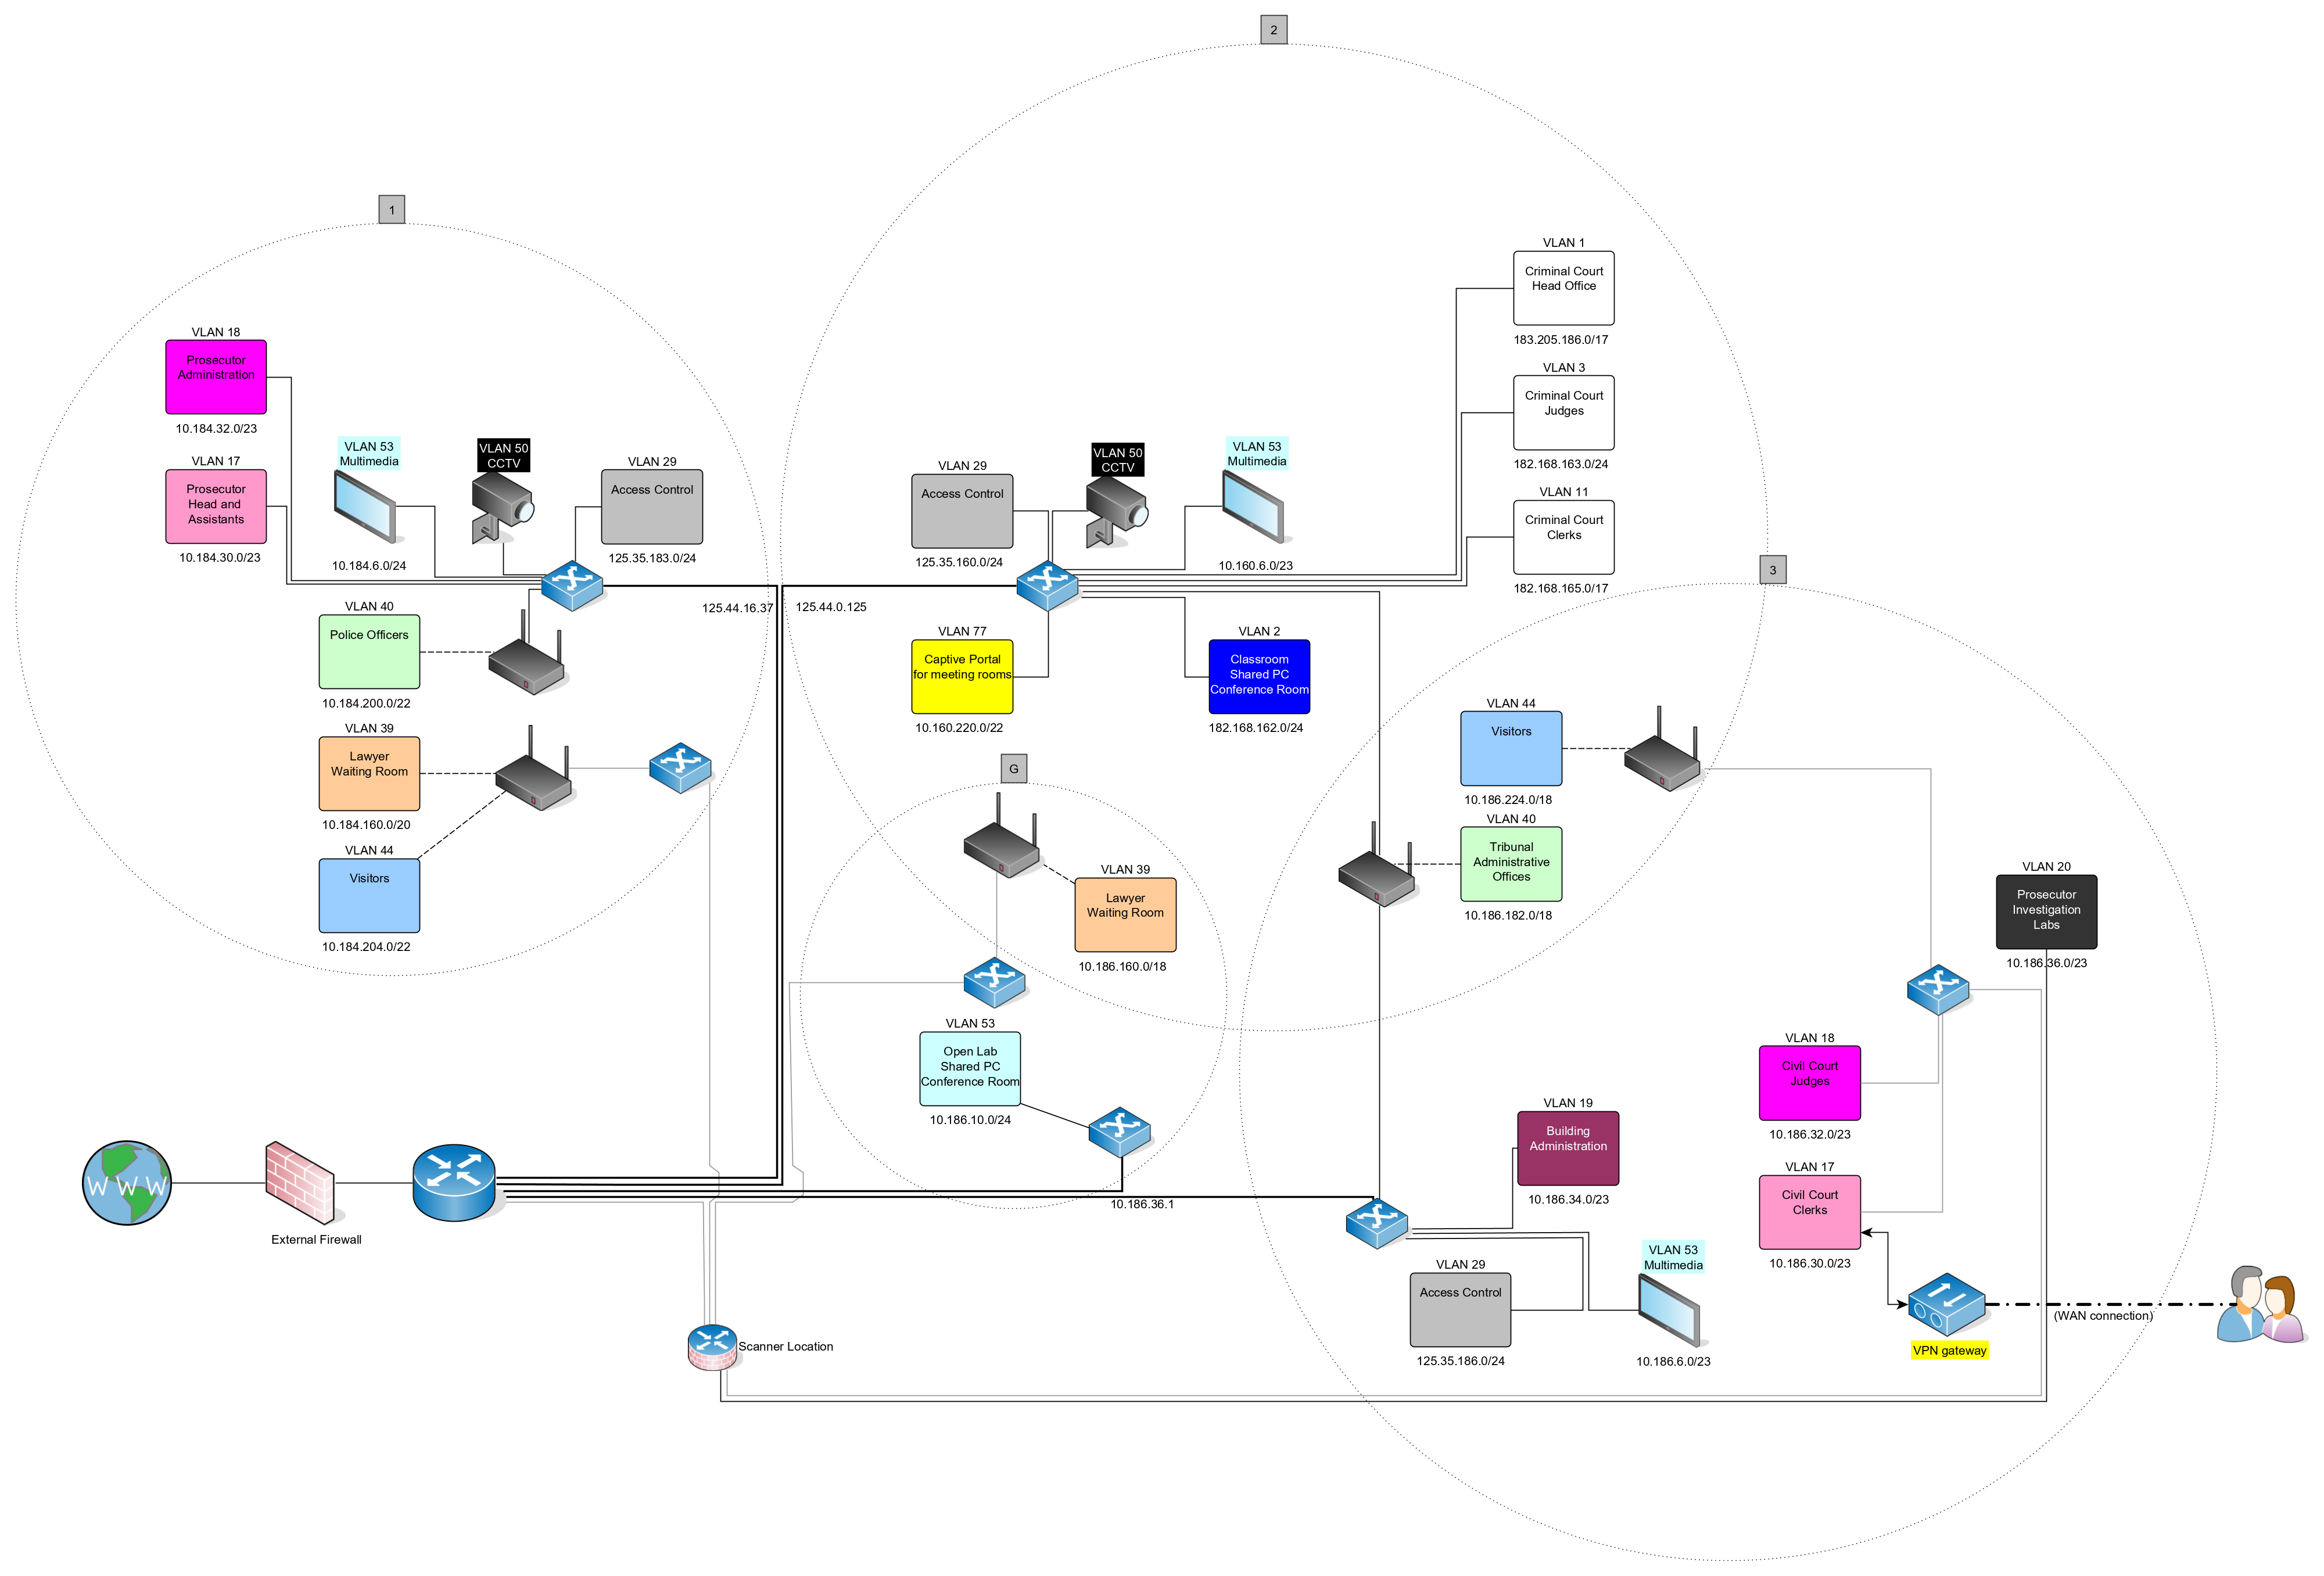
\includegraphics[width=\textwidth]{drawable/rete.png}
	\caption{Network diagram based on the Tribunal's provided scan.}
	\label{fig:initial-network}
\end{figure}

\clearpage